\documentclass[hidelinks,english]{article}

\usepackage{graphicx}
\usepackage{grffile}
\usepackage[T1]{fontenc}
\usepackage{babel}
\usepackage{wrapfig}
\usepackage{hyperref}

\date{\today}

\graphicspath{{Pictures/}}
\begin{document}	
	\begin{titlepage}
		\pagenumbering{gobble}
		\begin{figure}[!t]
			
\includegraphics[width=\linewidth]{up_logo.png}
		\end{figure}
		\vspace*{\stretch{1.2}}
		\begin{center}
			\huge{COS 786: Distributed and Parallel Computing\\}
			\huge{Project Documentation}\\
			\vspace{10mm}
			\huge{Armand Maree}\\
            \huge{\texttt{12017800}}
		\end{center}
		\vspace{15mm}
		\begin{center}
			Department of Computer Science, University of Pretoria
		\end{center}
		\vspace*{\stretch{2.0}}
	\end{titlepage}
	\newpage
	\tableofcontents
	\newpage
	\pagenumbering{arabic}
	
	\section{Introduction} 
		\paragraph\indent
		This document will discuss the various techniques used to implement the pirate distributed system.
        
	\section{Program Start Up} 
    	\subsection{Automated}
        	\paragraph\indent
            In order to execute all the clue solving pirates and the quarter master in one go, execute the \textit{run.bash} file. This will start the quarter master and $x$ clue solving pirates, where $x$ is the number of logical cores on the machine. Since all the programs will use the same terminal window the initial output might be cluttered initially, but this will settle down once the clue solving actually starts.
        \subsection{Manual}
          \subsubsection{Quarter Master (QM)}
              \paragraph\indent
              In order to start up the quarter master simply run the following command from a Linux terminal:
              \begin{center}
                  ./quartermaster.py --first --host <local IP>
              \end{center}
              \paragraph\indent
              From this point on this program will wait for incoming connections and manage all communication from the various other programs.

          \subsubsection{Clue Solving Pirates}
              \paragraph\indent
              To start up a new pirate program to solve clues, run the following command from a Linux terminal:
              \begin{center}
                  ./pirate.py --host <QM ip> --port <QM port>
              \end{center}
              \paragraph\indent
              The pirate will automatically connect to the quarter master specified. If no parameters are specified it will connect to localhost:40000.

              \paragraph\indent
              Once the pirate has connected to the quarter master, the quarter master will send all the clues and all the solved clues to the pirate. The \textit{pirate.dat} and \textit{ship.dat} file is also sent to the pirate. This is done in order to allow Rummy to be in the same state on another system should the current quarter master go offline. Once this has happened the new pirate is synchronized to the network and will start solving clues. Details on this will be discussed later.
    
	\section{Initial Crew} 
		\paragraph\indent
        When the quarter master starts up, it asks Rummy for 10 pirates. The pirates that Rummy maintains (i.e. the pirates that give Rummy clues) is regarded as separate from the pirates that the quarter master maintains (i.e. pirates that solve clues). This means that new clue solving pirates can connect at any stage of the clue solving process and do not have to wait for a new pirate to be allocated by Rummy.
    
	\section{Clue Distribution} 
		\paragraph\indent
        Any clue can be handed out to any pirate at any stage. This means that should one pirate be significantly slower than the other, it will not impact the performance of the whole system by holding on to a set of clues. This means that a slight increase of network traffic will occur, however, it will help the system to not be as heavily affected by slower pirates.
        
    \section{Communication}
    	\paragraph\indent
        Communication between the various programs were implemented using sockets. In order to reduce network traffic during the clue solving period the following enhancements have been made:
        \begin{enumerate}
        	\item When a program signs on to the network the current clue set is shared with it. This means that a once off big data transfer is done and from there only small messages have to be transferred. This also have some other error detection benefits that will be discussed later.
            \item All the information that relate to changes in the system are sent in batches. The batches are sent only when a clue solving pirate is idle. This means that occupied pirates cannot saturate the network while idle pirates have to wait for new instructions.
        \end{enumerate}
        
    \section{Leadership}
    	\paragraph\indent
        A central program called the quarter master is used to facilitate a star network between all the other programs. At all stages a quarter master has to be present in the system. A failure in this program will cause to entire system to halt. Recovery from this will be discussed later.
        
    	\paragraph\indent
        The quarter master is responsible for the communication between all of the other programs and Rummy. It also maintains a synchronized state between all the programs.
        
    \section{Corruption}
    	\paragraph\indent
        Corrupt pirates will cause the system to have to redo several clues during the problem solving process. After all the clues for a map has been done, the quartermaster evaluates the corruption of every pirate. If it is more than 10\% the pirate is removed from Rummy's crew. 10 new pirates are recruited once there are no pirates left on the crew. This is because the pirate recruitment process is time consuming.
        
	\section{Networking} 
		\paragraph\indent
        The whole system was implemented in such a way that it is able to run completely over a network and does not depend at all on a single global synchronous clock or shared memory. In figure \ref{piratesNetworkingFigure} is an example where two remote (completely different sites connected via the Internet) pirates, indicated with red boxes, connected to the quarter master and one local (on the same computer) pirate, indicated with a yellow box, connected to the quarter master.
        
        \begin{figure}[!h]
			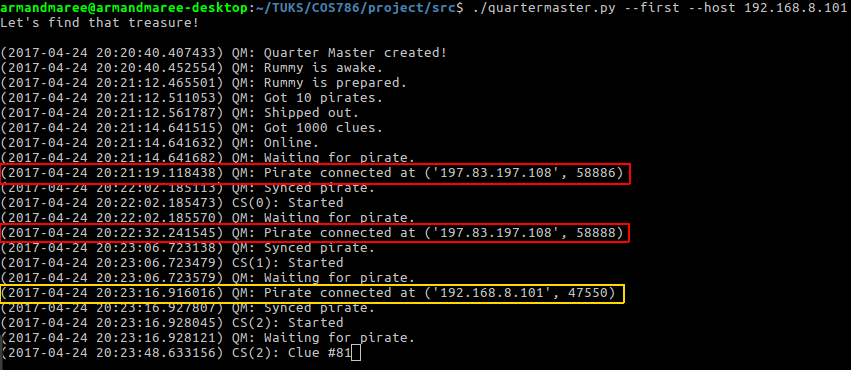
\includegraphics[width=\linewidth]{pirates.png}
            \caption{Example execution of two remote pirates and one local pirate.}
            \label{piratesNetworkingFigure}
		\end{figure}
        
    \section{Protocol}
		\paragraph\indent
        As soon as a clue solving pirate is synchronized to the network, the pirate will request a clue from the quarter master. The quarter master will respond with an index that corresponds with the clue that the pirate has to solve in the clues list that was synchronized when it connected initially. The pirate then solves the clues and sends the solved clue back to the quarter master and receives a new index in return which it has to solve. This process is repeated over and over until all the clues are solved.
        
		\paragraph\indent
        Once the quarter master receives a new solved clue, it broadcasts this clue to all other pirates on the network. When a pirate receives this solved clue, it saves it in its local memory. The reason for this is for fault recovery and is discussed in the next section.
        
		\paragraph\indent
        When a new clue solving pirate connects/disconnects to/from the quarter master, it broadcasts this information to all other pirates. Since this event does not occur very often it has minimal effect on the speed of the clue solving. This disconnect does not have to be graceful process, a sudden unexpected disconnect is handled in the same manner.
        
    \section{Fault Recovery}
    	\subsection{Pirate Faults}
			\paragraph\indent
            When a  clue solving pirate encounters some fault and this causes it to crash, the quarter master will broadcast to the remaining pirates which pirate is no longer part of the network and the other pirates will remove it from their memory. Should a point be reached where no pirate is connected to the quarter master, it will simply wait for new pirates to connect to resume the clue solving operation.
            
			\paragraph\indent
            When a pirate crashes the current map will never be able to be solved since the clue assigned to the pirate cannot be recovered. To overcome this, the clue that the pirate was supposed to solve is added into a recycle list as soon as the quarter master detects a failure in one of the pirates. This list has priority and will be picked up by the next pirate that requests a clue from the quarter master.
            
        \subsection{Quarter Mater Faults}
			\paragraph\indent
            Since the pirates rely on the functionality of the quarter master, the entire process stops as soon as the quarter master fails. In order to continue solving clues a new quarter master has to be spawned. 
            
			\paragraph\indent
            As the pirates connect to the quarter master initially they receive an ID. This ID is also broadcasted to the other pirates. When the quarter master fails, the pirate with the smallest ID number will start a new quarter master and connect to it. All other pirates will wait for the new quarter master to be spawned and then connect to it. the new quarter master's output will be logged to the \textit{qm.log} file. Since the IP address of the pirates are also broadcasted when the pirate connects, the pirates can connect to quarter masters on different servers on the fly. Pirates will attempt to connect to the new quarter master 20 times with 5 second delays between each attempt. If all 20 attempts fail the pirates will attempt to connect to the pirate with the second smallest ID. This process ensures that should multiple pirates disconnect along with the quarter master, the remaining pirates will attempt to reconnect to the remaining ones. 
            
			\paragraph\indent
            When the new quarter master has started up, it is synchronized to the network, similar to the way a pirate is synchronized, and then the clue solving continues.
            
    \section{Multithreading}
    	\paragraph\indent
        The only multithreading that was used was to facilitate the communication between the pirates and the quarter master. Since sockets were used, it was necessary to separate each pirate into it's own thread in order to be able to accept new connections continuously.
        
    \section{Execution Results}
    	\paragraph\indent
        The clue solving process takes about 2 hours, virtually on the dot, with 6 pirates running on a 6 core CPU. Due to all the fault recovery mechanisms in place, some performance was sacrificed.
    
    	
\end{document}